\documentclass{acmsiggraph}               % final

%% These two line bring in essential packages: ``mathptmx'' for Type 1
%% typefaces, and ``graphicx'' for inclusion of EPS figures.


\usepackage[utf8]{inputenc}
\usepackage{graphicx}
\usepackage{url}
\usepackage{times}
\usepackage{float}

%% Paper title.

\title{Polyspasm}

%% Author / Affiliation (single author).

%%\author{Roy G. Biv}
%%\affiliation{Allied Widgets Research\thanks{email:roy.g.biv@aol.com}}

%% Author / Affiliation (multiple authors).

\author{Jesper Öqvist \texttt{<jesper@llbit.se>}}

\affiliation{Lund University\\ Sweden}


%% Keywords that describe your work.
\keywords{Graphics Demo}

%%%%%% START OF THE PAPER %%%%%%

\begin{document}

\DeclareGraphicsExtensions{.png}


\maketitle

\section{Introduction}

The Polyspasm demo was created for the course project in EDAN35 High
Performance Computer Graphics in late 2012.  The demo features the typeface
Pusselbit, music by lft and parts of a Minecraft map by oldshoes.

In this report I present some of the graphics techniques used in the Polyspasm
demo.  I also list the libraries used and reflect briefly on the final result.

\subsection{Goals}

The goal of the course project was to implement at least two different
real-time graphics technique. My initial goals for Polyspasm was to render 3D
text and implement a fire effect and water effect on that text.

I have implemented these two initial effects, as well as a couple additional
effects.

\section{Code, Libraries and Assets}

All code for the project was written in C++ and GLSL.

There are about 4400 lines of C++ code \footnote{Line count obtained using
David A. Wheeler's \emph{SLOCCount}} and about 1300 lines of GLSL shader code.

The code quality is in places slightly embarrassing. The time constraints for
the project necessitated quick and dirty code. If I had more time to work on
the project I would have implemented my own matrix stack and cleaned up the
code a bit.

As it stands the code uses deprecated GLSL variables to access the OpenGL
matrix stack. It's not ideal and it's not pretty, but it works.

I believe that all of the shaders should work in GLSL 1.3.

\subsection{Libraries}

I used my own True Type Font library, cTTF, which is written in C. The cTTF
library was used to parse, interpolate and triangulate typefaces.

In addition, the following 3rd party libraries were used:

\begin{itemize}
	\item Simple DirectMedia Layer
	\item OpenGL
	\item The OpenGL Extension Wrangler Library
\end{itemize}

\subsection{Assets}

These art assets are used in Polyspasm:

\begin{itemize}
	\item A typeface called Pusselbit that I created in 2011.
	\item The song \emph{Kung Fu Goldfish} by Linus ``lft'' Åkesson.
	\item The Minecraft map \emph{Broville v10} by oldshoes.
\end{itemize}

\section{Effects}

In this section I will try to briefly describe how each of the effects in
Polyspasm work.

\section{Console}

The console effect and fire effect are my favorite effects in Polyspasm.  I'm
fond of the console effect because I spent the most time on making it synch up
nicely with the music. It is the first effect to appear, and is used to display
the title animation.

When I started toying around with GLSL for the project I had an idea that I
would like to render text that first appears to be just flat, ordinary text,
but the camera would zoom in and reveal it to actually be extruded 3D text.

To make the text appear flat I first set the view angle $\theta$ very small, at
1 degree.  The view angle is increased over time, until it reaches 107 degrees.
In order to keep the text size constant over that interval I scale the camera
distance by $1/\tan{\theta}$.

To add visual interest I made the text green, kind of inspired by an oldschool
terminal. I also added Gaussian blur to give it that nice glow it has. To make
the background less bland I put a texture behind the text, inspired again by an
oldschool terminal -- the texture is meant to look sort of like scanlines.
I also added a vignette effect in the Gaussian blur shader.

The Gaussian blur is implemented in two fragment shaders which first perform
a horizontal blur, and then a vertical blur. The horizontal blur shader renders
to an FBO which is sent as a sampler to the vertical blur shader.

The console effect is animated using a vertex shader that displaces the
vertices in the text, and a fragment shader that warps the scanline texture.

A GLSL PRNG I found online is used to get some randomness in the displacement
shaders. The PRNG I used was found at
\url{http://www.steelratsoftware.com/articles/71-glsl_rnd.html}. I used the
simpler version as it did not require the \texttt{floatBitsToUint} built-in
function which is not available prior to GLSL 3.3 I believe.

\begin{figure}[H]
    \centering
    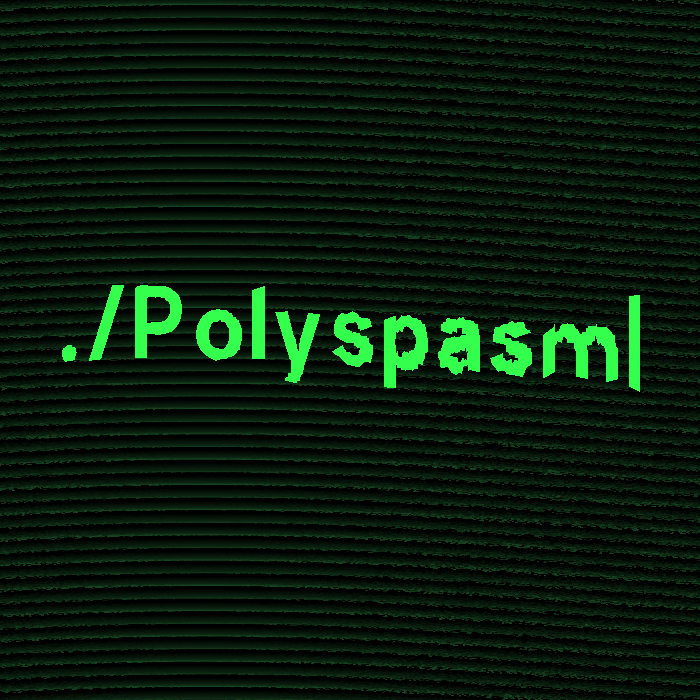
\includegraphics[width=0.7\columnwidth]{console0.png}
    \caption{Console effect without blur and vignette.}
\end{figure}

\begin{figure}[H]
    \centering
    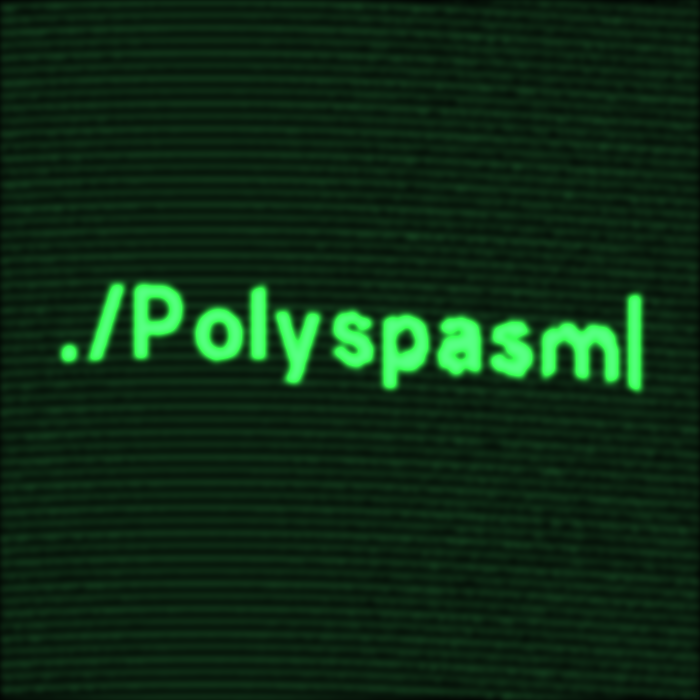
\includegraphics[width=0.7\columnwidth]{console1.png}
    \caption{Console effect with Gaussian blur.}
\end{figure}

\begin{figure}[H]
    \centering
    
\includegraphics[width=0.7\columnwidth]{console2.png}
    \caption{Console effect with Gaussian blur and vignette.}
\end{figure}

\subsection{Ray Tracing}

In the second scene of the demo the camera flies over a Minecraft landscape.
The sky changes color to the melody of the music, switching from blue to
yellow and back.

The Minecraft landscape is a part of the Minecraft map Broville v10 which I
exported using my Minecraft mapping tool Chunky
\footnote{http://chunky.llbit.se}. It was exported in a binary octree format
which I hastily wrote a parser for in C++. The octree data is packed into a 2D
texture with 32-bit integral internal format. I first tried to use a 1D
texture, but the texture size limit prevented me from using that approach. In
order to send as much data as I needed to my shader I had to wrap it into a 2D
texture.

The octree data is rendered using a fragment shader called ``pt''. This is
really a simple implementation of a path tracer in GLSL.  Since the camera is
constantly moving in the second scene we never get to see the path tracer
compute more than one sample per pixel. However, in scene four the camera is
stationary and we can see the path tracer accumulate samples. Scene four
uses a different part of the Broville map.

Samples and sample counts are stored in an FBO with a \verb'GL_RGB16F' color
attachment for accumulated sample values and a \verb'GL_R8UI' color attachment
for sample counts.

I found that it was too cumbersome to render a full FBO worth of samples per
frame. Instead I select random points on the unit sphere and extrude a quad for
each point which is then rendered using the path tracing shader. This means
that there are sometimes overlapping quads which causes redundant work, but on
the other hand I avoid rendering the full frame, so it's a worthwhile tradeoff.

Randomly discarding samples was very inefficient. I think the quad sampling
technique works well because it better utilises ray locality and doesn't start
a lot of shaders for pixels that will just be discarded.

In the end I like the sort of distortion that occurs due to the random quad
sampling, so it stuck.

\begin{figure}[H]
    \centering
    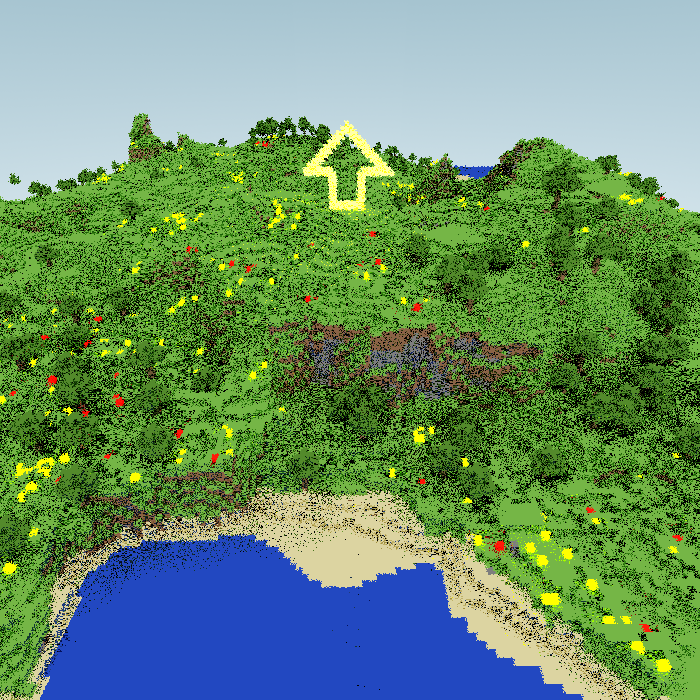
\includegraphics[width=0.7\columnwidth]{raytrace.png}
    \caption{A frame from the second scene.}
\end{figure}

\subsection{Fire}

I like this effect because I think it looks really cool and it was fun to
implement.

The fire is simulated using a fluid simulator.  My fluid simulator
implementation is based on chapter 38 of GPU Gems 1 by Mark J. Harris
\cite{fernando2004gpu}.  There is source code provided in the article that I
could use with a few modifications. I ignore boundary conditions, and instead
just shrink the viewport so that I never touch the outermost pixels in the
advection, buoyancy or force addition steps. I skipped the viscous diffusion
step, and added buoyancy to get the flames to rise.

Force addition is the step where hot air, or flames, are added to the fire
simulation. To get the outlines of the text I rendered the normals of the text
to an FBO and then used a Sobel operator shader for edge detection. Using the
output of the edge detector directly would cause constant ``flow'' of fire from
the edges of the text. This ends up looking okay, but to make it look really
good the fire should look like it is burning unevenly, kind of like the embers
in a fireplace.

To get the uneven burn effect I used simplex noise to modulate the intensity
of the flames added in force addition. I also used a simple three by three
box filter to blur the sharp edges that are produced by the edge detector.

I implemented the 2D simplex algorithm, an improvement of classic 2D Perlin
noise, using Stefan Gustavsons excellent article on the subject:
\url{http://www.itn.liu.se/~stegu/simplexnoise/simplexnoise.pdf}.

After the fluid simulator has simulated one timestep I render the flames using
a shader that maps the floating point values in the temperature buffer using
a color gradient that shifts from white to orange to red to black.

\begin{figure}[H]
    \centering
    
\includegraphics[width=0.7\columnwidth]{fire0.png}
    \caption{Edge detected text.}
\end{figure}

\begin{figure}[H]
    \centering
    
\includegraphics[width=0.7\columnwidth]{fire1.png}
    \caption{Edge detected text modulated by simplex noise.}
\end{figure}

\begin{figure}[H]
    \centering
    
\includegraphics[width=0.7\columnwidth]{fire2.png}
    \caption{Resulting fire effect when the output of the
	edge detector is used as a temperature source.}
\end{figure}

\subsection{Water}

The water effect was really tricky, and I am not satisfied with the result.

Originally I wanted to do refraction correctly in the text. It became difficult
to make the refraction technique look good and believable.  I myself don't
really have intuition for what water refraction should really look like and
on top of that it's so unusual to see water in such solid well-defined chunks,
so I could never fool myself that it was supposed to look like water.
In the end I cheated and just implemented translucency. I think it looks better
than with the refraction. It still doesn't really look like water.

I used a shader to do texture lookups in a skybox for the transmitted light
rays. I used simplex noise to displace the direction of the transmitted rays.
This gives sort of a ripple effect on the surface of the text. The text is
rendered to two different FBOs before the translucency is rendered using
backface culling for one and frontface culling for the other. The difference
between closest front-facing surface and closest back-facing surface is
computed using the depth buffers of both FBOs and this value is used to
modulate the blueness of the water effect.  It's hardly noticeable in the end,
but if you look hard you can see that the text is sort of more translucent
close to the edges.

\begin{figure}[H]
    \centering
    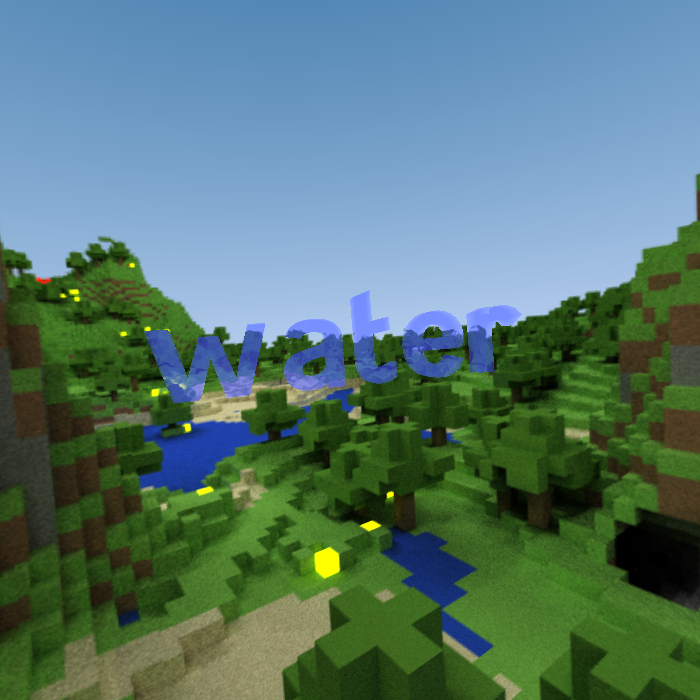
\includegraphics[width=0.7\columnwidth]{water.png}
    \caption{The final water effect.}
\end{figure}

\section{Black-and-White}

There is an effect near the end of the fourth scene and throughout the final
scene where the world is black-and-white. This is the effect of applying the
Sobel operator mentioned previously to the path traced skybox.

In the final scene I just draw the normals for the surfaces of the song credits
in front of the skybox before applying the Sobel operator.

\section{Conclusion}

Overall I am very pleased with my demo, although I wish I had time to clean up
the code and implement my own matrix stack. Yet, I am pleased that the project
is done now so that I can concentrate on other stuff.

I spent a lot of time synchronizing the demo with the music. In the end I did
not have enough time to do that properly, so the synchronization is pretty
bad near the end. I could have done that better but again, I did not have
enough time.

It was really fun to implement the fire effect with the fluid simulation and
simplex noise. It was really satisfying to see that it turned out so well,
when I was worried I would not have time to implement it at all.

The water effect would probably have been a bit nicer if I had added some
specular highlights to the ``waves''.

\bibliographystyle{acmsiggraph}
%\nocite{*}
\bibliography{project}
\end{document}
